\chapter{Fabrication \& Sensing of Input Devices}


\begin{quote}
In addition to the profound repercussions these technologies
will likely have on the manufacturing industry, the
democratization they enable promises to unleash creativity
and innovation at a level comparable to those brought about
by the personal computer and the internet.

--- Catarina Mota, \emph{The Rise of Personal Fabrication}
\end{quote}

Our goal is to fabricate input device prototypes whose properties we can predict and sense. This chapter will describe the design space of such devices, covering today's digital fabrication machines, the materials they can process, the properties inherent in those materials, potential characteristics of fabricated objects, and sensor varieties. Further, we will discuss potential ``links'' between object properties and sensors: for example, some processes can create tine structures (cantilevered beams); when struck, these tines vibrate at frequencies determined by their geometry and material, and their vibrations can be sensed and decoded by a microphone.

\valkyrie{Hmm, writing this made me realize that maybe we need to describe more than just the pairing between fab characteristics and sensors? Maybe: 1) user action 2) mechanism 3)material characteristic 4) sensable change from coupling 1 to 2 5) sensor selection. You do this at the very end of this chapter. Maybe we want to bring this into the intro somehow?
For Midas: 
1) touch 2) none 3) conductivity 4) capacitance 5) capacitive touch chip
For Sauron:
1) physical movement (push/slide/rotate); 2) 3d printed mechanism 3) rigidity, color 4) visual motion 5) camera
For LAmello
1) physical movement 2) plucking mechanism 3) controlled tine geometry 4) vibration 5) microphone} \valkyrie{My intuition is that making so many levels would be complicated, especially since we have a "none" as one of the steps on one of our projects.}

\section{Definitions}

First, we briefly define words and machines that will be discussed in this chapter and the remainder of the thesis.

\emph{additive fabrication} : in additive fabrication, material is deposited and a shape is built up.

\emph{subtractive fabrication} : a subtractive fabrication process removes material to create a form. Excess material may be reused in another project or discarded.

\emph{3D printer} : a 3D printer is one of a class of machines that additively create a three-dimenstional model from one or more materials.

\emph{FFF} : FFF (fused-filament fabrication) 3D printers lay down material by melting and depositing a filament in a precise pattern.

\emph{model material} : model material is the substrate that the final object is made from

\emph{support material} : many modern 3D printers are capable of laying two types of materials, model material and a secondary, sacrificial material that can support overhangs in the model while printing, then be removed.

\emph{SLA} : SLA (stereolithography) printers use a bath of UV-curable polymer and a controllable UV laser. The laser "draws" each layer on the polymer, causing photopolymerization where it strikes. Excess material is simply poured out for reuse.

\emph{SLS} : SLS (selective laser sintering) 3D printers contain a bed of material (e.g., metal powder) which is compacted and formed into a solid mass of material by heat and/or pressure without melting to the point of liquefaction. Excess material can be brushed off and reused.

\emph{Polyjet} : Polyjet printers have print heads similar to those of inkjet printers which sweep across the build area depositing material. Following the printer head is a UV light, which cures deposited material droplets.

\emph{vinyl cutter} : a vinyl cutter subtractively processes 2D materials with a 2-axis knife blade, cutting patterns into them. Vinyl cutters are typically used for thin, flexible materials.

\emph{laser cutter} : a laser cutter has a 2-axis laser for processing flat materials. Laser cutters can cut or engrave into materials, and are often used for rigid materials $1</4$ inch thick. Some have rotary attachments for etching on circular surfaces like the outside of a glass.

\emph{CNC router} : a CNC router uses a 3-axis rotary mill to cut through thick, rigid materials, like wood or certain metals. Some CNC routers are portable and can attach to many materials, while some are stationary with beds into which material is loaded.

\emph{CNC mill} : a CNC mill is a multi-axis machine which subtractively creates a 3D shape from a block of material, usually metal or wood.

\section{Digital Fabrication}

Digital fabrication machines are those which can take as input a digital design file, in 2D, 2.5D, or 3D, and output a physical realization of that design. A design created in a computer-aided design (CAD) tool is processed by a computer-aided manufacturing (CAM) tool to create machine instructions to generate the object. This workflow stands in contrast to traditional crafting techniques (which do not require machine code) as well as manufacturing techniques (which require ``tooling'' for each design created). The true power of digital fabrication lies in its ability to create unique objects with each machine run \emph{without} the extensive setup and tooling necessary to change the product created by, for example, an injection moulding machine. This comes with the blessing and curse that each instance of an object costs as much to manufacture as the one before it, but allows for variations between instances without additional cost. For example, even makers can now create custom 3D printed replacement joints and prosthetics that fit particular bodies, e.g., a new hand for a young girl who wants to do monkey bars \cite{myers-sophie}.

The joint interests of industry, academia, and hobbyist makers have led to a flourishing ecosystem of digital fabrication and rapid prototyping (RP) machines. These machines describe a continuum from simple vinyl cutters that can subtractively create 2-dimensional stickers to sophisticated multi-material 3D printers that can create multicolor and conductive designs where the designer has full 3D control over the external and internal geometry of object. These machines allow their manufactured products to achieve various material and structural properties. We examine materials properties of common digital fabrication inputs (see Figure \ref{table:fab-properties}), as well as the machines that can process them and the compositional properties they make possible (see Figure \ref{table:materials-machines}).

\begin{figure}
\centering
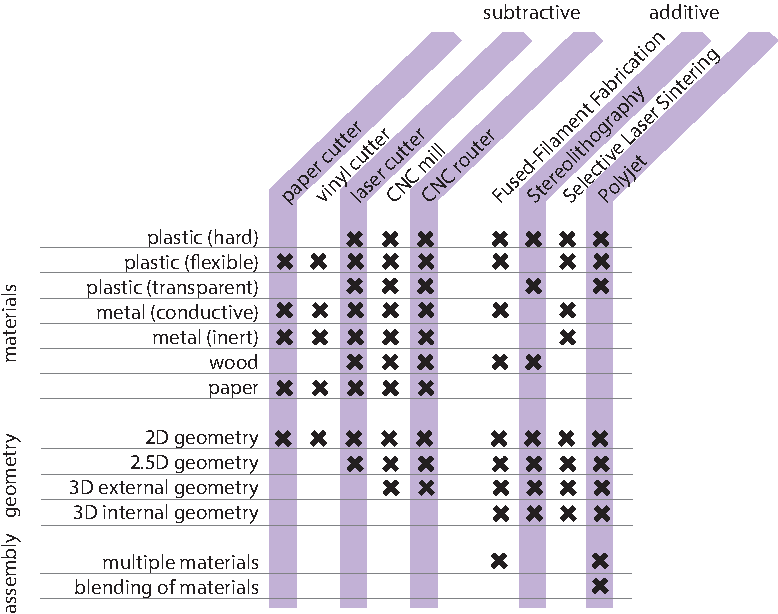
\includegraphics[width=3in]{figures/fab-properties.pdf}
\caption{The most common materials processed by digital fabrication machines, including plastic and wood, have wildly different realizable characteristics.}
\label{table:fab-properties}
\end{figure}

\begin{figure}
\centering
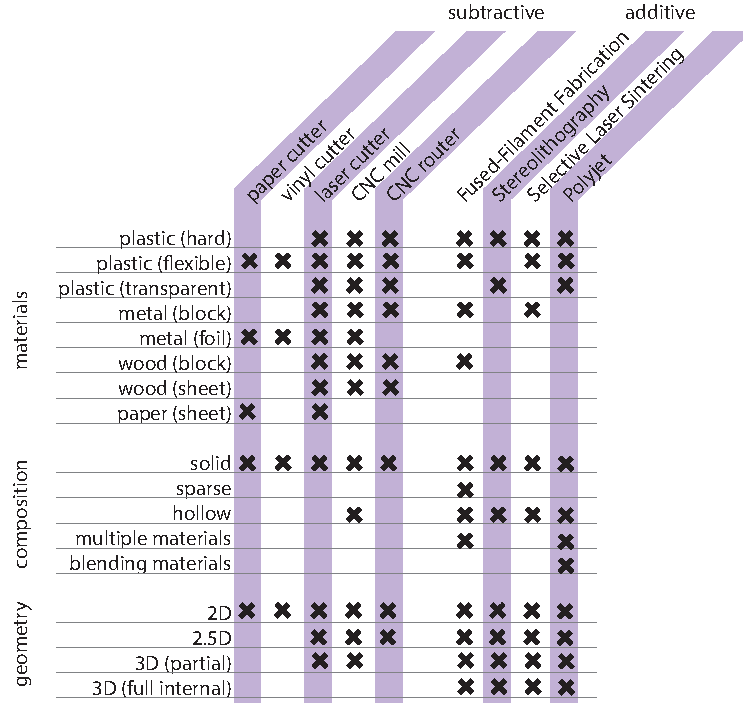
\includegraphics[width=5in]{figures/materials-machines.pdf}
\caption{Additive and subtractive RP machines each have their own sweet spots of operation. Subtractive tools can process more types of materials, but additive ones offer more compositional flexibility.}
\label{table:materials-machines}
\end{figure}

\subsection{Geometry Fabrication}

Digital fabrication machines can support any complexity of geometry, from 2D images on paper (as an inkjet printer produces) to 3D projections of 4D objects (like Shapeways's Klein bottles printed in steel) (see Figure \ref{fig:range}). We describe the possibilities for the various geometries, as well as machines that could produce them. Note that we list machines at the edge of their range: for example, a CNC mill (listed under 3D external) can also make 2.5D or 2D objects.

\begin{figure}
\centering
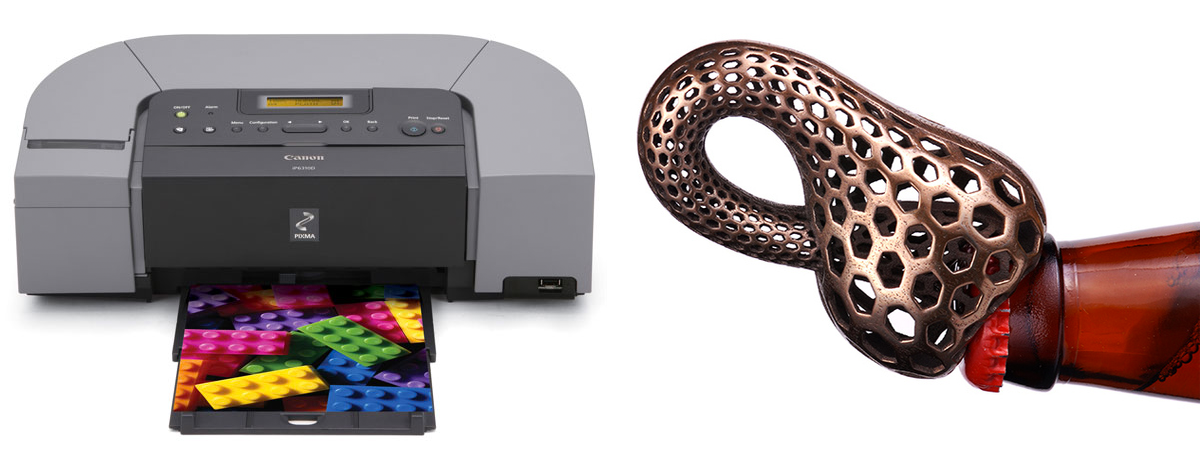
\includegraphics[width=4in]{figures/range.png}
\caption{The range of objects produceable via digital fabrication is huge: from 2D images on paper (left, from Amazon), to 3D projections of 4D objects (right, from Bathsheba on Shapeways).}
\label{fig:range}
\end{figure}

\subsubsection{2D geometry}

2D geometry lies flat on a surface, but can manifest as an image printed on paper, a sticker cut from vinyl, or a barcode engraved on granite. Machines that support 2D geometry fabrication include vinyl and paper cutters, as well as inkjet printers.

\subsubsection{2.5D geometry}

A slight jump from 2D is 2.5D: a 2D shape with additional \emph{depth} information. The canonical machines to create 2.5 objects are 3-axis CNC routers, which mill away material from the surface and can take multiple passes for deeper features.

\subsubsection{3D external geometry}

Features like overhangs can be challenging to mill using a 2.5D machine, as subtractive techniques require that the machine tool has unobstructed access to the surface to be milled. Creating such features on a 2.5D machine may require reorienting an object several times. Some machines are capable of creating arbitrary 3D external geometry, including overhangs, without manual reorientation of a part. This is can be accomplished by machines that use both a model material and a sacrificial support material: combining the two materials permits overhangs that may not be possible using only a single material. However, removal of this support material can be challenging, depending on the process used. (See \cite{savage-sot} for a more complete treatment of support material and removal techniques.) 3D printers can produce overhang geometry by laying support material as a part of each 2D object slice, and 5-axis CNC mills can produce overhangs via automatic object reorientation.

\subsubsection{3D internal geometry}

Full control over internal geometry can only be executed via additive manufacturing, and it allows for designed cavities, mechanisms, textures, and more on the interior of objects manufactured in a single pass. Again, this is typically executed by machines that lay sacrificial support material.

\subsection{Materials and Properties}

Beyond geometric properties, the types of materials that can be processed using the various additive and subtractive RP machines is equally broad. Each material lends itself to certain types of manipulations, and different materials may be more easily formed by different machines.

\valkyrie{I wonder if properties would be the better top-level organizing principle, rather than materials:
so: Appearance: opaque-translucent-transparent
Appearance: color-no color
Rigidity: rigid-flexible
Conductivity: isolator-resistor-conductor ?
Material fill : solid-sparse-hollow
Then you could have process x material gives rise to certain properties. add color}

\subsubsection{Plastic (hard)}

Hard plastics---including thermoplastics like acrylonitrile butadiene styrene (more commonly known as ABS) and polylactic acid (known as PLA)---are the materials du jour in the maker community. They come in the form of heatable, extrudable filaments for FFF machines (e.g., Makerbot, Printrbot, Reprap, uPrint). Hard plastics can also be additively processed with other 3D printing techniques, for example photocure plastics in polyjet machines (ABS-like and Vero series for Objet machines) and SLA machines (methacrylates in Form1), or thermoset plastics like epoxy in research systems (e.g., Harvard's system \cite{compton-epoxy}).

Hard plastics can also be subtractively processed through milling and laser cutting, although many plastics are unsafe for laser vaporization (e.g., ABS plastic emits chlorine gas when lasercut).

\subsubsection{Plastic (flexible)}

Flexible plastics are less common than hard ones, though there are some notable materials here: thermoplastic polyurethane (sold as Ninjaflex) is a filament-style flexible material for use in FFF machines, and some polyjet machines likewise have support for flexible plastics (e.g., Tango series for Objet).

Subtractive processing for flexible plastics is possible, though may be more challenging due to different shear parameters than stiffer materials. PVC plastic in the form of vinyl sheets can be cut to shape with a vinyl cutter.

\subsubsection{Plastic (transparent)}

Transparent plastics are not yet available for most maker-class machines, though many SLA-processed resins are optically translucent and polyjet machines offer optically transparent plastics (e.g., VeroClear for Objet). Laser cutters are suitable for processing sheets of transparent acrylic, as well.

\subsubsection{Metal (conductive)}

Conductive metal is relatively simple to process subtractively (e.g., milling circuitboards on a CNC router), even by vinyl cutters which can cut thin metal foils. Certain conductive metals, e.g., steel, can be directly laser-sintered in a high-heat process. Conductive-impregnated filaments for FFF machines do exist in limited use, but they are typically based on graphene (carbon) rather than metals. The new Voxel8 FFF 3D printer \cite{voxel8} uses a silver-based material for conductive purposes.

\subsubsection{Metal (inert)}

Inert metals are processed in essentially the same ways as conductive metals, although they have not been engineered for use in FFF filaments.

\subsubsection{Wood}

Wood-type materials are most commonly subtractively processed (e.g., by CNC routing). Newer processes are available to add wood in the form of sawdust to FFF-compatible filaments (e.g., woodfill by colorfabb), and also to laser sinter with wood chips \cite{materialise-wood}.

\subsubsection{Paper}

Paper is trivially subtractively processed. None of the four main 3D printing methods can use paper-based materials, though one subtractive/additive method uses stacks of cut paper to create 3D paper models (e.g., MCor IRIS).

\subsection{Assembly Characteristics}

\valkyrie{This paragraph is very abstract. I’m not sure what to take away from it.}

Additive digital fabrication methods offer significant freedom in terms of assembly methods. Many types of printers can use multiple materials for the same part, and even blend them. This allows for fabricating parts of multiple colors or shore (hardness/softness) values, or simply creating parts which are pre-assembled and interlocked after support material is removed. 

\section{Single-Sensor Sensing Techniques}

One key research area in Human Computer Interaction is designing new techniques and algorithms to help computers accept human input. Thus, while many of the input techniques here could be used in, for example, machine-to-machine communication, we describe how a person's actions might create a usable control signal.

\subsection{Single-sensor Motivation}

Why use a single sensor? To reduce time spent on each iteration of a prototype performing assembly and calibration, we aim to allow users to fabricate an object and snap on a single sensing module. In the future, it would be interesting to explore multi-sensor modules (e.g., modern smartphones have magnetometers, capacitive screens, microphones, cameras, and more), however as initial work we are exploring one sensor at a time.

\subsection{Sensor Types}

A ``single sensor'' can take many forms, ranging from a humble switch which opens and closes to a high-speed video camera which captures 2D visual information at 1000Hz to an accelerometer measuring G-forces in 3 directions.
%\valkyrie{Card, et al., provide an analysis of the space of input devices based on what is sensed: position, $\Delta$position, angle, $\Delta$angle, force, $\Delta$force, torque, and $\Delta$torque \cite{card-input}. We use this to frame our discussion, but include additional senseable aspects: identity (of a user), bend/$\Delta$bend, and ???. We could also include, for example, \emph{intent}, which is the input of NLP voice systems like Siri, however these types of non-physical input are challenging to conceive of as a part of a physical input device and we therefore ignore them for now.}
As they represent a vast array of possibilities in terms of actions sensed, physical phenomenon, and more, and there are multiple ways of organizing sensors for discussion purposes. We use the hierarchy proposed by the Modern Sensor Handbook \cite{citation needed!}: it arranges sensors by actions sensed, which neatly aligns with our user-driven prototypes. In these categories, we discuss thirty common varieties of sensors, like capacitance sensors, hall effect sensors, voltage sensors, temperature sensors, and pulse sensors.

The major categories in the Modern Sensor Handbook are
\begin{itemize}
    \item occupancy and motion
    \item position, displacement and level
    \item velocity and acceleration
    \item force, strain and tactile
    \item pressure
    \item flow
    \item acoustic
    \item humidity/moisture
    \item light detectors
    \item radiation detectors
    \item temperature
    \item chemical sensors
\end{itemize}


\valkyrie{The physical effects that are the basis of sensors include: capacitance, magnetism, induction, resistance, piezoelectric effect, pyroelectric effect, hall effect, thermoelectric effect, ...}

\subsection{Contact sensors}

Contact sensors are mainly used either to sense contact with an object (in the case of switches, capacitance, flex, or force sensing) or used while in contact with an object to sense other forces on it (as in load sensors, accelerometers, and gyroscopes). This kind of sensor can directly sense physical human input.

\subsection{Non-contact sensors}

Non-contact sensors, like the contact variety, can directly sense physical human input. They can, however, do so without being in contact with the human or the input device being sensed. Non-contact sensors rely on waves (e.g., visible for cameras, audible for microphones, radio for RFID) or fields (e.g., magnetic for hall effect) to sense interactions. 

\subsection{Electrical sensors}

Electrically-based sensors like volt-meters and potentiometers can be used as tools for internal monitoring of a circuit, but are also able to sense human input. A potentiometer attached to a knob, for example, will change its resistance value as a user manipulates the knob.

\subsection{Environmental sensors}

Environmental sensors, like pressure and altitude sensors, are generally used to sense ambient details, as opposed to human input. However, certain ambient details can be modified by human presence or activity: for example, human users can output sweat senseable via humidity sensors, and human presence may raise the local temperature of a area.

\subsection{Biological sensors}

Human bodies perform several semi-controllable processes: hearts beat, brains think, etc. Biological sensors detect these processes. They can be used for input by humans, but the user may require some training to be competent at creating distinct signals.

\section{Promising Overlaps}

The spaces of both machines and sensors are vast, so we describe some ways to think about combining them to actually fabricate sensing objects.

\begin{figure}
\begin{adjustbox}{addcode={\begin{minipage}{\width}}{\caption{%
      Lining up the possibilities of fabricatable properties with sensor types, we can see several areas that are promising for further exploration. We also identify pairings that have been explored previously, as well as pairings explored in this thesis. 1. Capricate \cite{schmitz-capricate}, 2. Flexibend \cite{chien-flexibend}, 3. Stane \cite{murray-smith-stane}, 4. Printed Optics \cite{willis-printedoptics}, 5a. Design by physical composition \cite{doering-composition}, 5b. Dynamic latex buttons \cite{harrison-buttons}, 6. Depth camera as touch sensor \cite{wilson-depthtouch}, 7. Pressure-sensing robot skins \cite{slyper-pressure}.
      }\end{minipage}},rotate=90,center}
      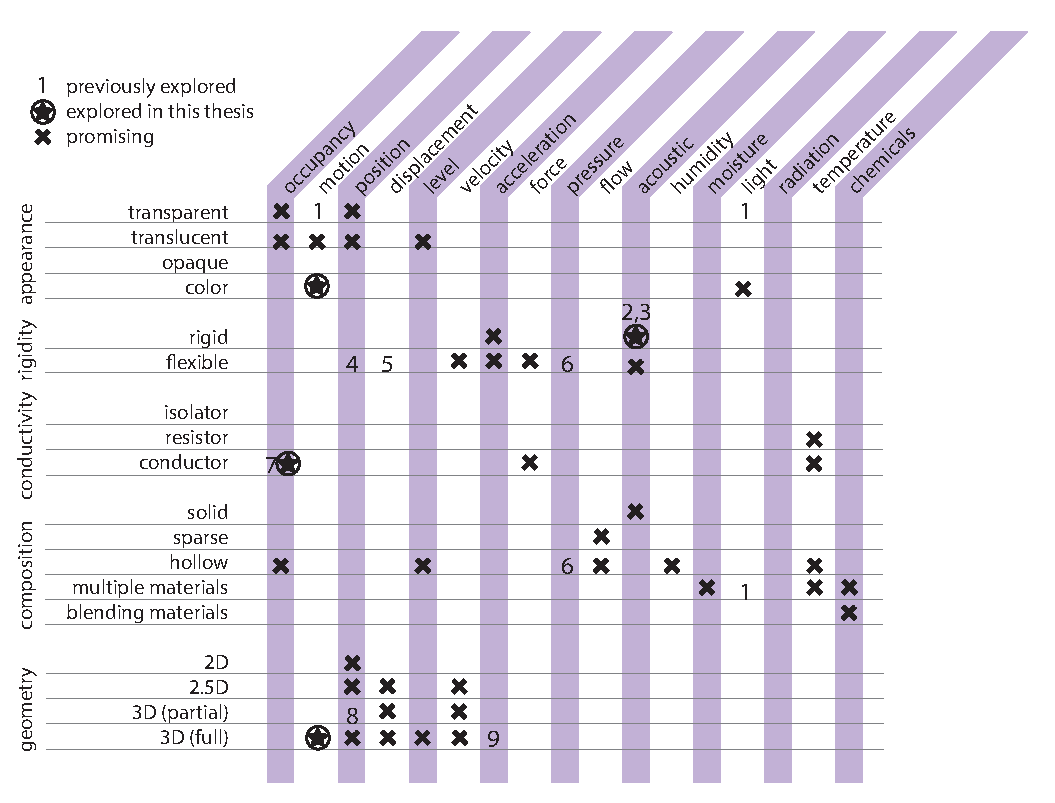
\includegraphics[scale=.75]{figures/sensing-fab.pdf}%
  \end{adjustbox}
\label{fig:sensing-fab}
\end{figure}

\subsection{Principles}
    
    Several principles guide our selections. Namely,
    \begin{itemize}
      \item for materials: \begin{itemize}
        \item the material ideally conducts (but at least does not insulate) the signal to be passed. For example, metal conducts electricity, and so is compatible with electrical sensing; paper conducts moisture, and thus could be used with humidity sensing.%; pulse can be sensed optically, so clear material may be compatible with pulse sensing.
        \item a user's manipulating the material should generate a control signal senseable using the given sensor. For example, bending a flexible plastic generates a signal detectable by a flex sensor. %\valkyrie{actually different from above?. yes.}
        \end{itemize}
      
      \item for geometry: \begin{itemize}
        \item geometry should work with the sensing abilities of a given technology. For example, an object with a solid core would not allow fluids to sense for particulate sensing; allowing 3D internal geometry would make this sensing possible.
        \item geometry needs to make it possible for a given type of signal to reach every part of an object without collision. For example, a camera inside a 3D object may require geometry modifications  or mirrors to see around corners. \valkyrie{still chewing on this one...}
        \end{itemize}
      
      \item for assembly characteristics: assembly characteristics of an object may be necessary in combination with particular materials properties to get additional sensing. For example, blending stiff and flexible plastics may allow for more unique degrees of sensing with a flex sensor. \valkyrie{still not clear after previous discussion of assembly techniques}
      
      %\item for sensors: to avoid complex machine learning, sensors should measure phenomena which can be mathematically modeled from digital design files. For example, the range from an ultrasonic rangefinder to a moving slider may be easier to model than the force generated by a user flexing a part with a Shore value of 35. \valkyrie{do we need this section? basically all the other sections reference sensor compatibility anyway.} \valkyrie{realistically, a caveat is that I know more about contact/non-contact/electrical sensors than I do about the other things. they are more commonly used in HCI as far as I'm aware, and maybe I just don't have the brain bendability to identify how they could be effectively leveraged using fab.}
    \end{itemize}
    
    These principles give rise to the \textbf{x}s marked in Figure \ref{fig:sensing-fab}.
    
\subsection{The Most Promising Overlaps}

    \valkyrie{choose a few things outside this thesis that we think are the best places to look next. blendable flexy materials + FSR. print electromagnets with conductive material, sense motion with gausssense (sensor block powers magnet channels??)}
    
\subsection{Overlaps Discussed in this Thesis}

    \subsubsection{Conductive Metal + 2D Geometry + Capacitive Sensor}
    
    Chapter 4 describes Midas, a technique for creating custom capacitive touchpads CNC cut from adhesive copper foil. These can be affixed to everyday objects and sensed using a single capacitive touch controller.
    
    \subsubsection{Hard Plastic + 2D/3D Geometry + Microphone}
    
    Chapter 5 describes Lamello, a technique for creating tines from hard plastic; when struck each tine vibrates at a characteristic frequency which can be classified using a microphone.
    
    \subsubsection{3D Internal Geometry + Camera}
    
    Chapter 6 describes Sauron, a technique leveraging arbitrary internal geometries to create mechanical input devices that can be sensed by a single embedded camera.